\chapter{Конструкторский раздел}

В данном разделе представлены схемы реализуемых алгоритмов и их модификации.

\section{Трудоемкость алгоритмов}\label{estimate}
Для получения функции трудоемкости алгоритма необходимо ввести модель оценки трудоемкости. Трудоемкость "элементарных" операций оценивается следующим образом:
\begin{enumerate}
	\item Трудоемкость 1 имеют операции:
	\begin{equation*}\label{math:simple}
		\begin{array}{cc}
			+, -, =, <, >, <=, >=, ==, +=, -=,\\
			++, --, [], \&\&, ||, >>, << \\
		\end{array}
	\end{equation*}
	\item Трудоемкость 2 имеют операции:
	\begin{equation*}\label{math:complex}
		*, /, \char`\\ , \%
	\end{equation*}	
	\item Трудоемкость конструкции ветвления определяется согласно формуле \ref{math:if}.
	\begin{equation}\label{math:if}
		f_{if} = f_{\text{условие}} + 
		\begin{sqcases}
			min\left(f_{true} , f_{false}\right) \text{ в лучшем случае,} \\
			max\left(f_{true} , f_{false}\right) \text{ в худшем случае.} \\
		\end{sqcases}
	\end{equation}
	\item Трудоемкость цикла расчитывается по формуле \ref{math:loop}.
	\begin{equation}\label{math:loop}
		f_{\text{цикл}} = f_{\text{инициализация}} + f_{\text{сравнение}} + N \left(f_{\text{тело}} + f_{\text{инкремент}} + f_{\text{сравнение}}\right);
	\end{equation}
	\item Трудоемкость вызова функции равна 0.
\end{enumerate}

\section{Трудоемкость алгоритмов}

\subsection{Классический алгоритм}

Пусть на вход алгоритму поступают матрицы $M_{left}$ и $M_{right}$ с размерностью $n \times m$ и $m \times q$. Тогда трудоемкость классического алгоритма определяется по формуле \ref{math:alg}
\begin{multline}\label{math:alg}
	f_{alg} = f_{{цикл_i}} = 2 + n\left(2 + f_{цикл_j}\right) = 2 + n\left(2 + 2 + q\left(2 + f_{цикл_k}\right)\right) = \\
	= 2 + n\left(2 + 2 + q\left(2 + +2 + 14 \cdot m\right)\right) \approx 14mnq = 14MNQ;
\end{multline}
\subsection{Алгоритм Копперсмита — Винограда}

Трудоёмкость алгоритма Копперсмита — Винограда состоит из:
\begin{itemize}
	\item создания и инициализации массивов MH и MV, трудоёмкость которого (\ref{for:init}):
	\begin{equation}
		\label{for:init}
		f_{инициализация} = M + N;
	\end{equation}
	
	\item заполнения массива MH, трудоёмкость которого (\ref{for:MH}):
	\begin{equation}
		\label{for:MH}
		f_{MH} = \frac{19}{2}MN +6M +2;
	\end{equation}
	
	\item заполнения массива MV, трудоёмкость которого (\ref{for:MV}):
	\begin{equation}
		\label{for:MV}
		f_{MV} = \frac{19}{2}QN +6Q +2);
	\end{equation}
	
	\item цикла заполнения для чётных размеров, трудоёмкость которого (\ref{for:cycle}):
	\begin{equation}
		\label{for:cycle}
		f_{cycle} = 16MQN + 13MQ + 4M + 2;
	\end{equation}
	
	\item цикла, для дополнения умножения суммой последних нечётных строки и столбца, если общий размер нечётный, трудоемкость которого (\ref{for:last}):
	\begin{equation}
		\label{for:last}
		f_{last} = 3 + \begin{cases}
			0, & \text{чётная,}\\
			16MQ + 4M + 2, & \text{иначе.}
		\end{cases}
	\end{equation}
\end{itemize}

Итого, для худшего случая (нечётный общий размер матриц) имеем (\ref{for:bad}):
\begin{equation}
	\label{for:bad}
	f =  f_{MH} + f_{MV} + f_{cycle} + f_{last}\approx 16 \cdot MNQ;
\end{equation}

Для лучшего случая (чётный общий размер матриц) имеем (\ref{for:good}):
\begin{equation}
	\label{for:good}
	f =  f_{MH} + f_{MV} + f_{cycle} + f_{last} \approx 16 \cdot MNQ;
\end{equation}


\subsection{Оптимизированный алгоритм Копперсмита — Винограда}

Оптимизированный алгоритм Винограда представляет собой обычный алгоритм Винограда, за исключением следующих оптимизаций:
\begin{itemize}
	\item вычисление происходит заранее;
	\item используется битовый сдвиг, вместо деления на 2;
	\item используется битовый сдвиг, вместо умножения на 2.
\end{itemize}


Трудоёмкость улучшенного алгоритма Копперсмита — Винограда состоит из:
\begin{itemize}
	\item создания и инициализации массивов MH и MV, трудоёмкость которого (\ref{for:impr_init}):
	\begin{equation}
		\label{for:impr_init}
		f_{инициализация} = M + N;
	\end{equation}
	
	\item заполнения массива MH, трудоёмкость которого (\ref{for:impr_MH}):
	\begin{equation}
		\label{for:impr_MH}
		f_{MH} =  \frac{13}{2}MN + 4M + 5;
	\end{equation}
	
	\item заполнения массива MV, трудоёмкость которого (\ref{for:impr_MV}):
	\begin{equation}
		\label{for:impr_MV}
		f_{MV} =  \frac{13}{2}QN + 4Q + 5;
	\end{equation}
	
	\item цикла заполнения для чётных размеров, трудоёмкость которого (\ref{for:impr_cycle}):
	\begin{equation}
		\label{for:impr_cycle}
		f_{cycle} =2 + M \cdot (4 + N \cdot (11 + \frac{Q}{2} \cdot 21));
	\end{equation}
	
	\item условие, для дополнения умножения суммой последних нечётных строки и столбца, если общий размер нечётный, трудоемкость которого (\ref{for:impr_last}):
	\begin{equation}
		\label{for:impr_last}
		f_{last} = 3 + 
		\begin{cases}
			0, & \text{чётная,}\\
			13MQ + 4M + 2, & \text{иначе.}
		\end{cases}
	\end{equation}
\end{itemize}

Итого, для худшего случая (нечётный общий размер матриц) имеем (\ref{for:bad_impr}):
\begin{equation}
	\label{for:bad_impr}
	f = f_{MH} + f_{MV} + f_{cycle} + f_{last} \approx 10.5MNK;
\end{equation}

Для лучшего случая (чётный общий размер матриц) имеем (\ref{for:good_impr}):
\begin{equation}
	\label{for:good_impr}
	f = f_{MH} + f_{MV} + f_{cycle} + f_{last} \approx 10.5MNK;
\end{equation}

\section{Схемы алгоритмов}
На рисунке \ref{fig:alg} приведена схема классического алгоритма умножения матриц. На рисунке \ref{fig:win-1} приведена схема алгоритма Копперсмита -- Винограда. Рисунок  
\ref{fig:win-2} демонстрируют схему оптимизированного алгоритма Копперсмита -- Винограда.\newpage

\begin{figure}[ht!]
	\centering
	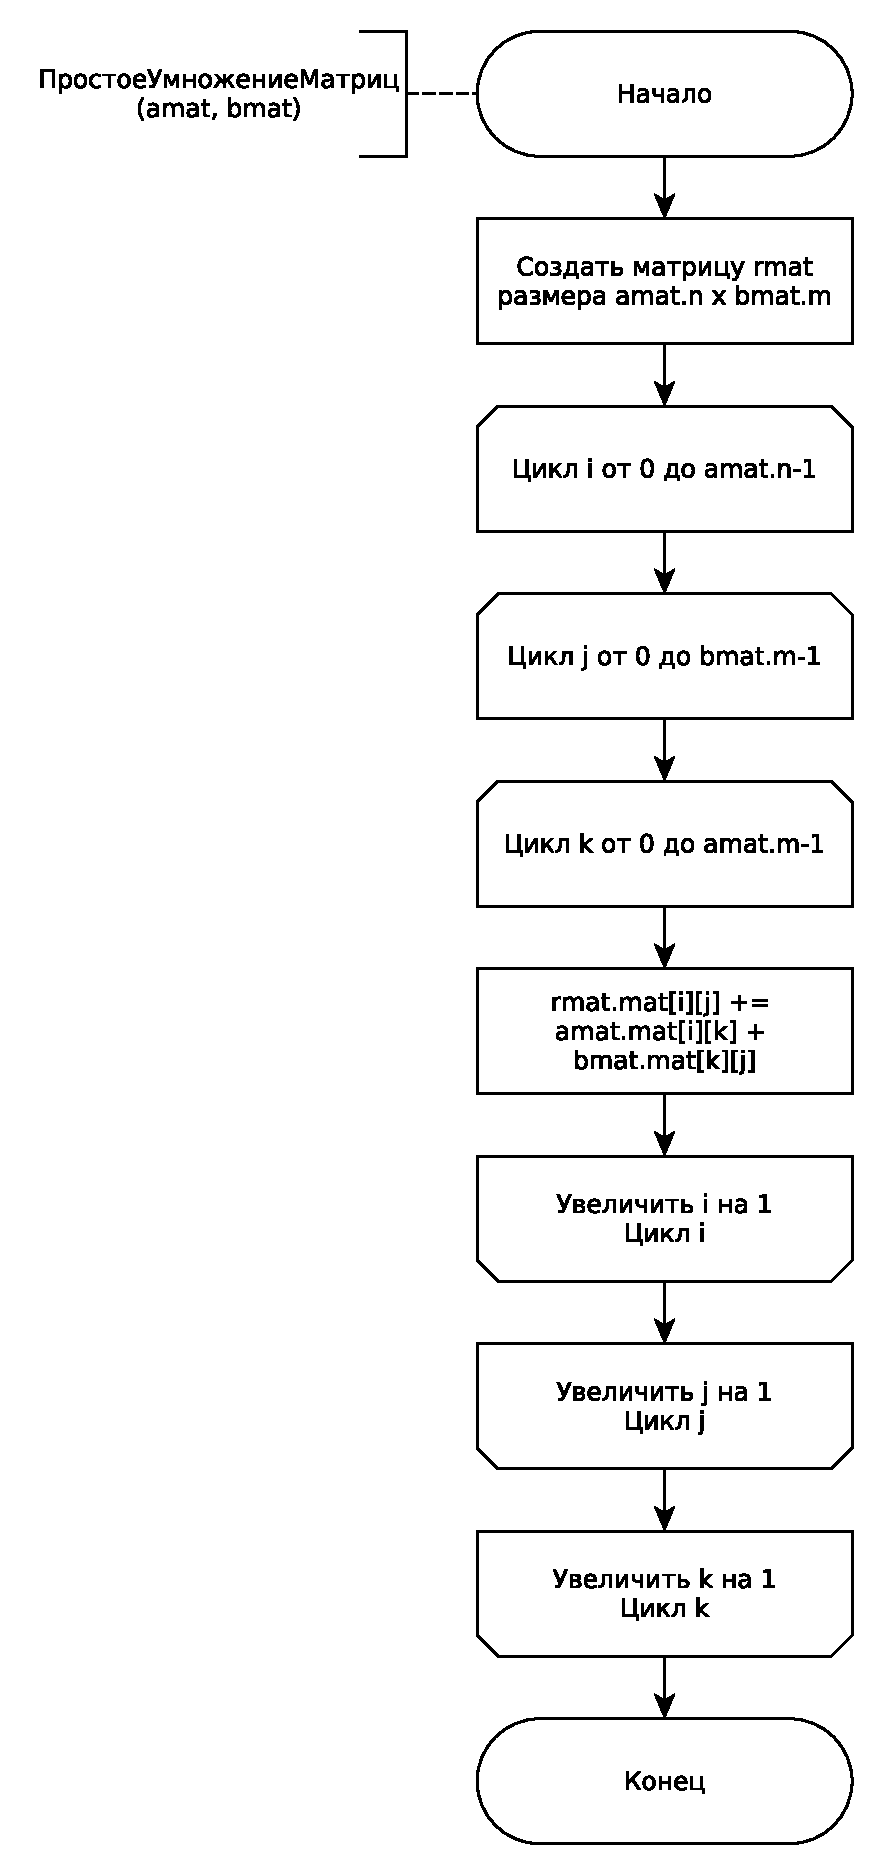
\includegraphics[width=0.65\linewidth]{assets/mtx-alg.pdf}
	\caption{Схема классического алгоритма умножения матриц}
	\label{fig:alg}
\end{figure}

\begin{figure}[ht!]
	\centering
	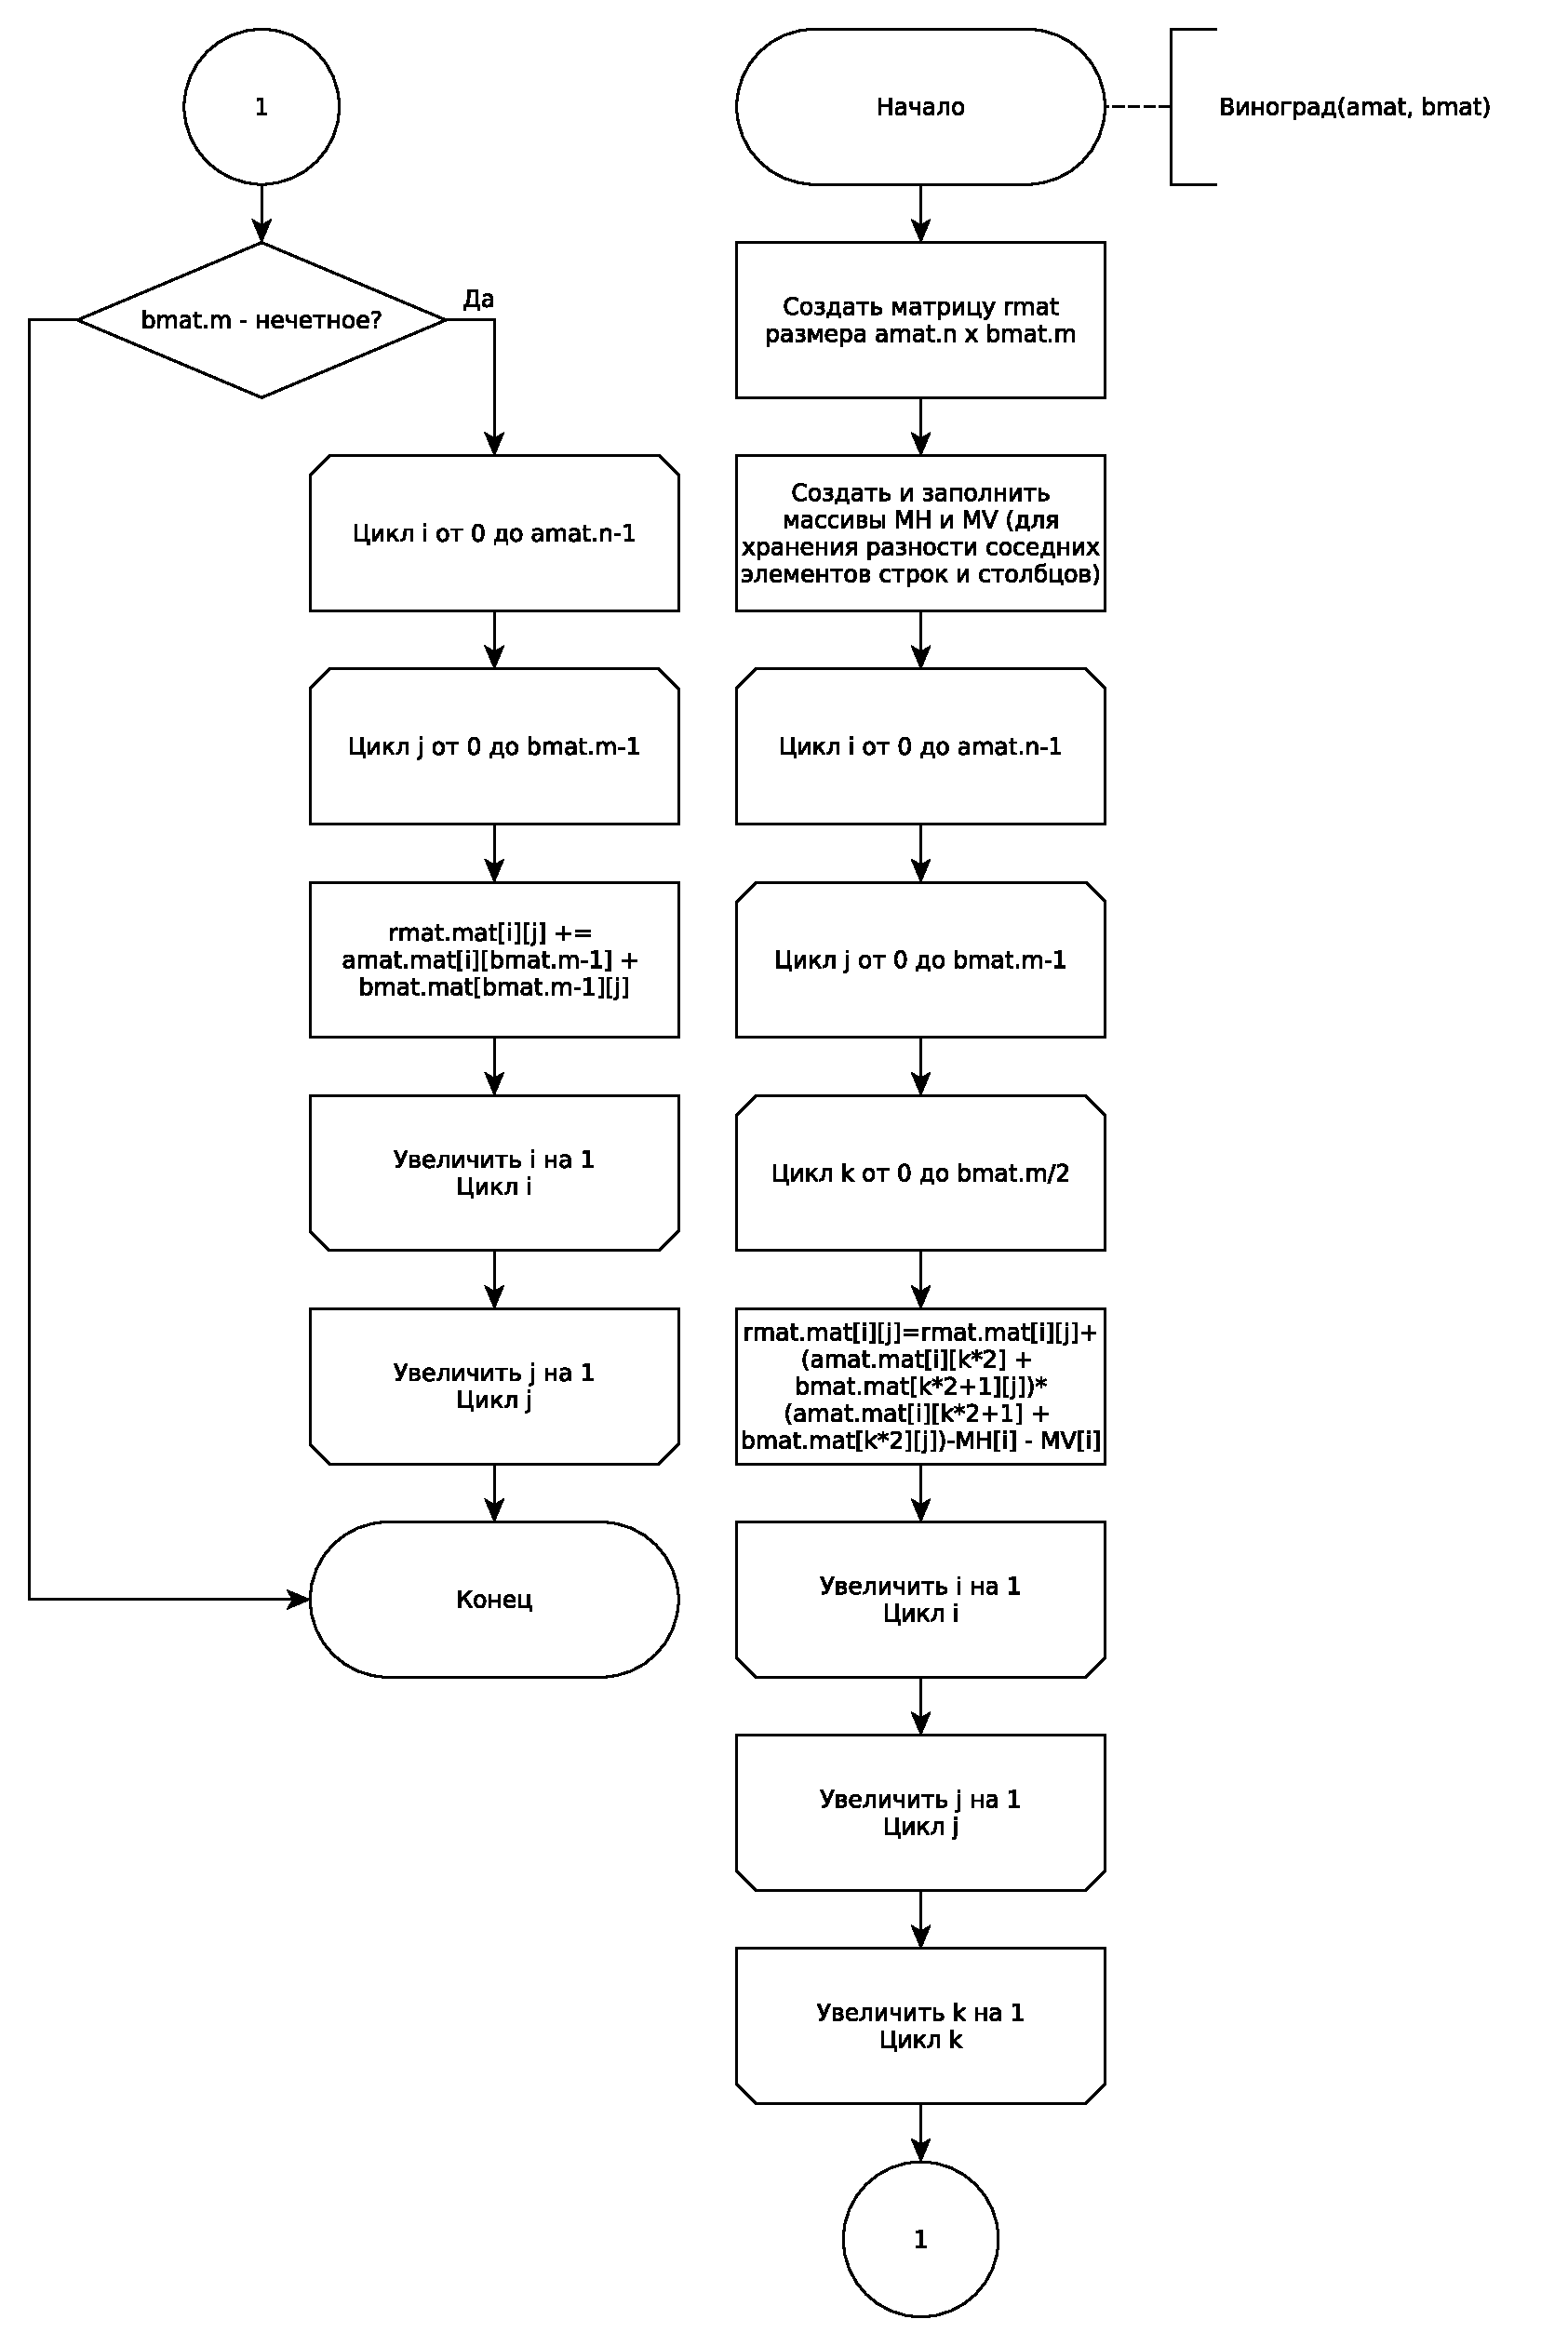
\includegraphics[width=0.90\linewidth]{assets/mtx-win1.pdf}
	\caption{Схема алгоритма умножения матриц Копперсмита -- Винограда}
	\label{fig:win-1}
\end{figure}

\begin{figure}[ht!]
	\centering
	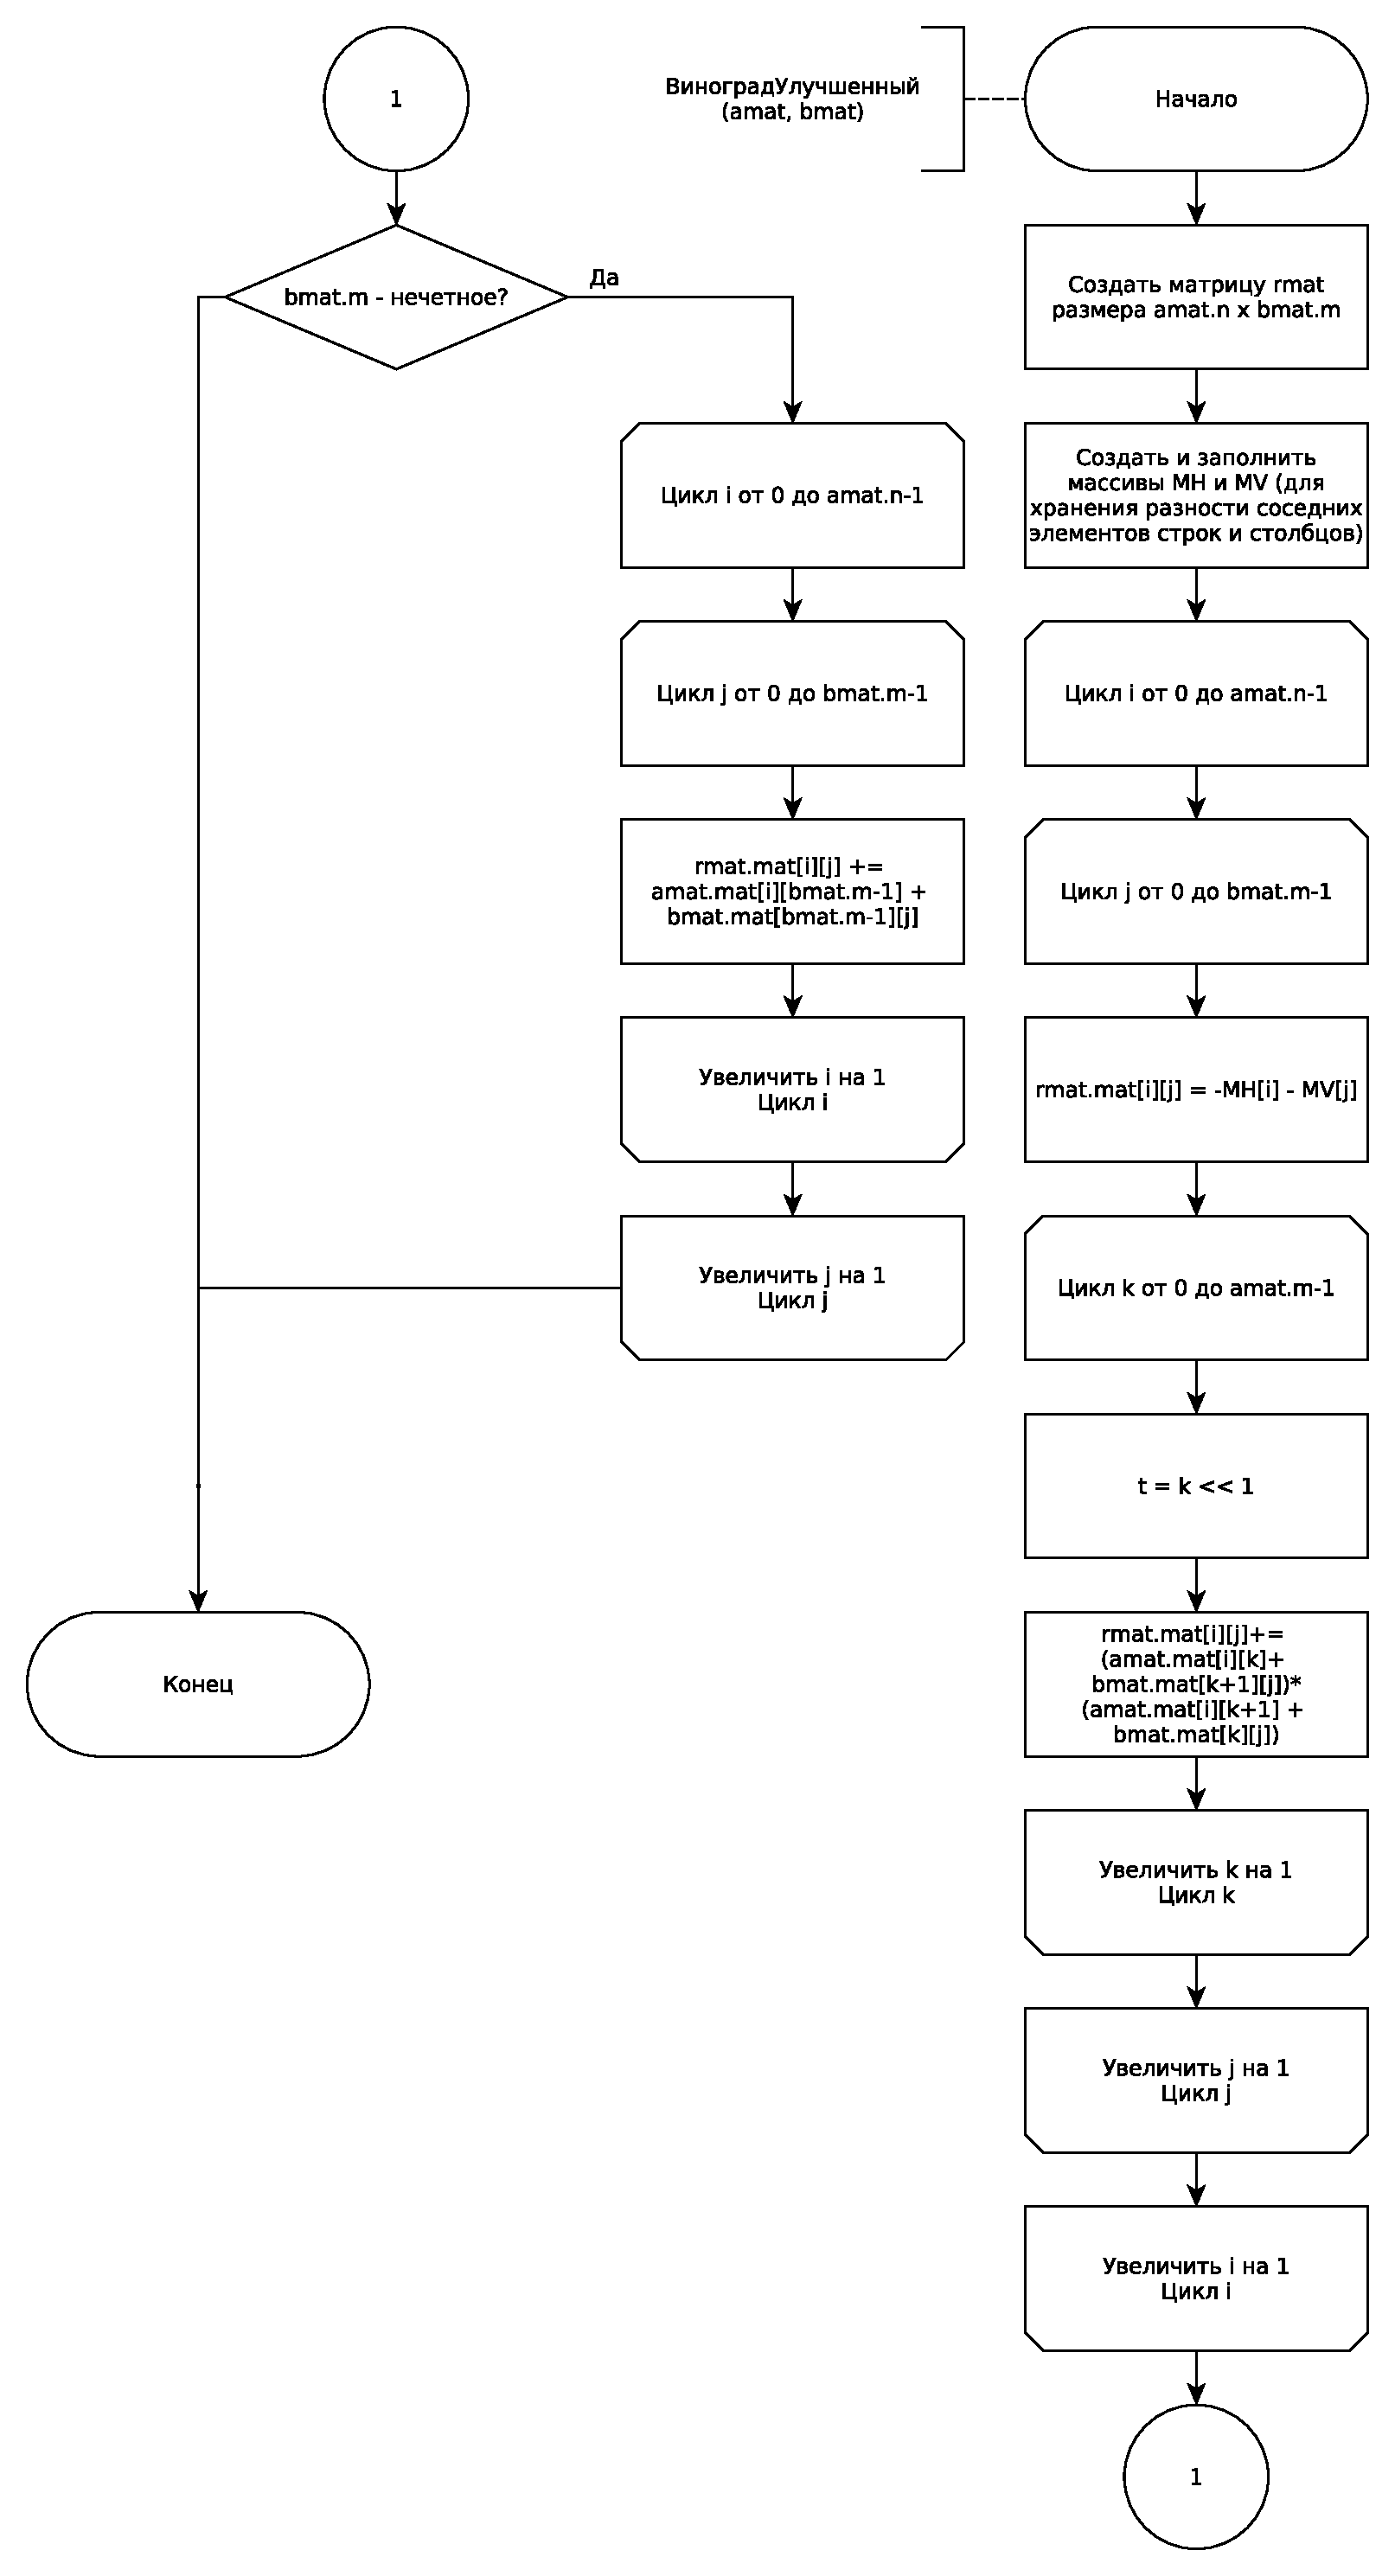
\includegraphics[width=0.82\linewidth]{assets/mtx-win2.pdf}
	\caption{Схема оптимизированного алгоритма умножения матриц Копперсмита -- Винограда}
	\label{fig:win-2}
\end{figure}

\newpage
\section*{Вывод}
Алгоритмы были проанализированы с точки зрения временных затрат. Было выявлено, что оптимизированный алгоритм Копперсмита -- Винограда работает в 1.5 раза быстрее, чем классический алгоритм Копперсмита-Винограда.


Были построены схемы алгоритмов. Теоретически были исследованы способы оптимизации алгоритма Копперсмита - Винограда. Было получено достаточно теоретических сведений для разработки ПО, решающего поставленную задачу.